\begin{center}
    %%%%%%%%%%%%%%%%%%%%%%%%%%%%%%%%%
    %%%%%%%%%%%% Moltres %%%%%%%%%%%%
    %%%%%%%%%%%%%%%%%%%%%%%%%%%%%%%%%
    \begin{tcolorbox}[colback=white, colframe=black, width=0.95\textwidth, arc=6pt, boxrule=1pt]
        \sectiontitle{Moltres}
        \sectioncontent{
            $S_N-D$ method for accurate time-dependent control rod modeling in Moltres,
            an open-source MOOSE application for the simulation of molten salt reactors \cite{park}.

            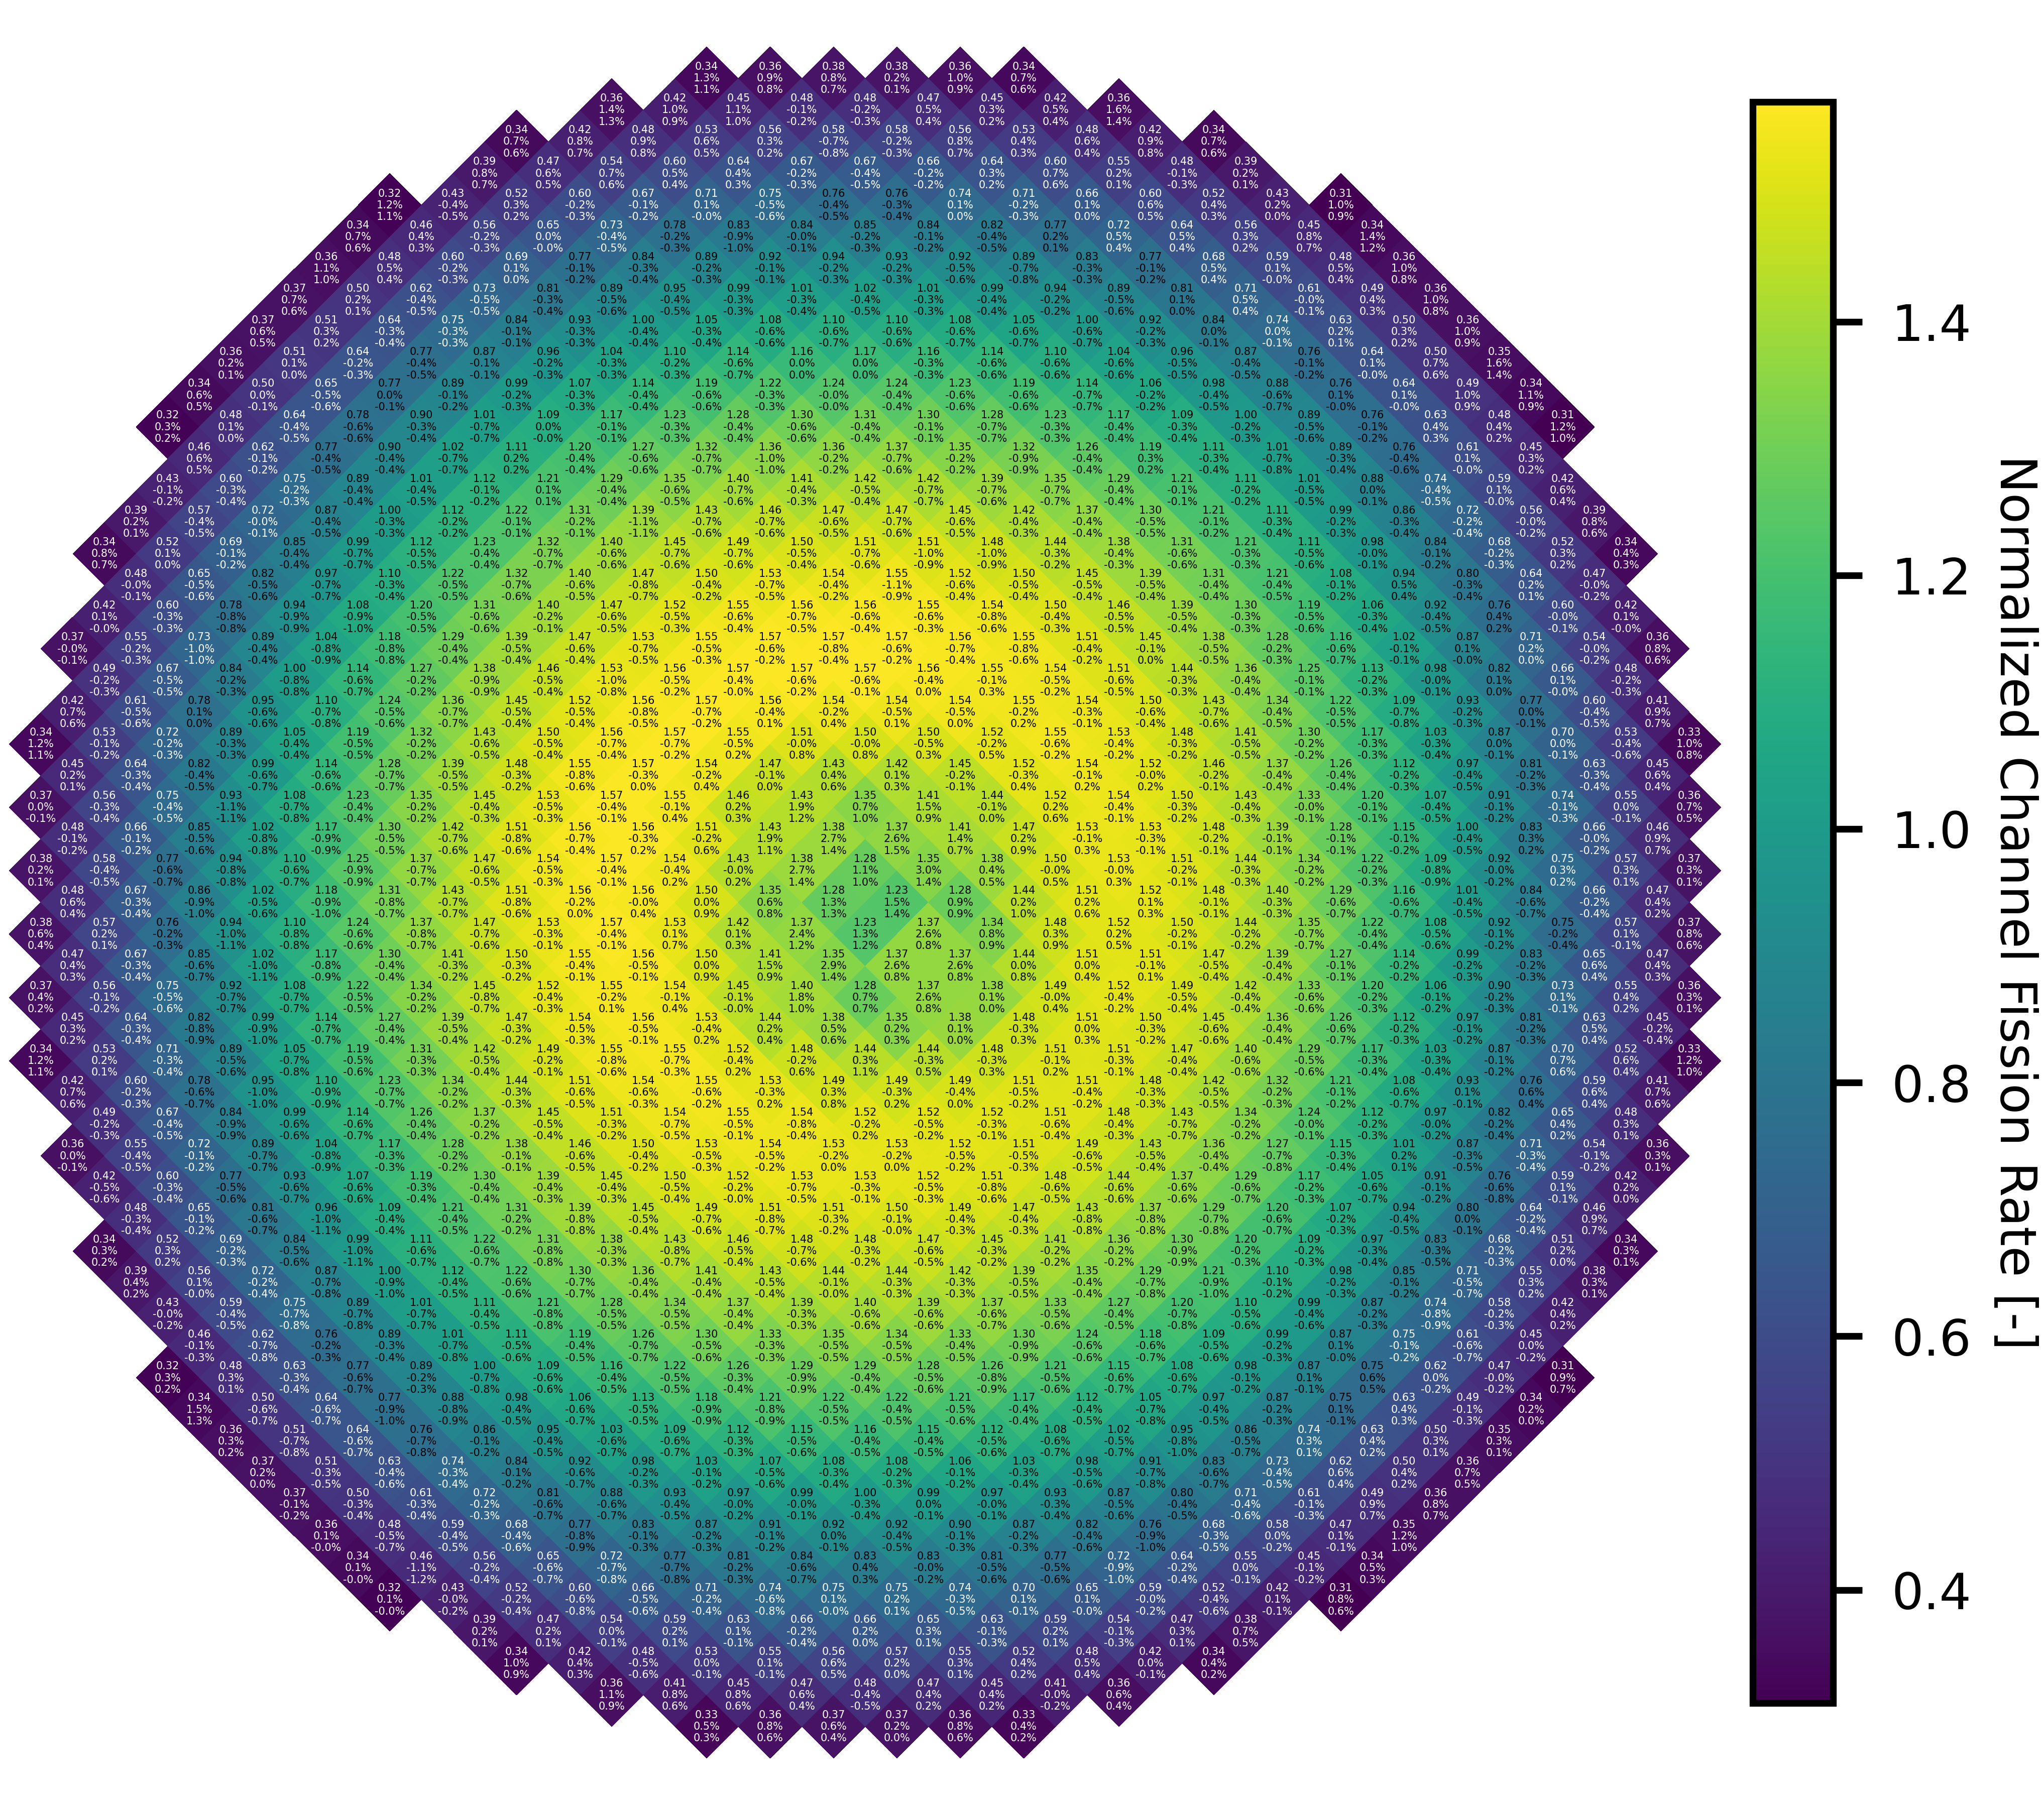
\includegraphics[width = .4\textwidth]{img/msre-full-0-power.png}
            \hspace{2cm}
            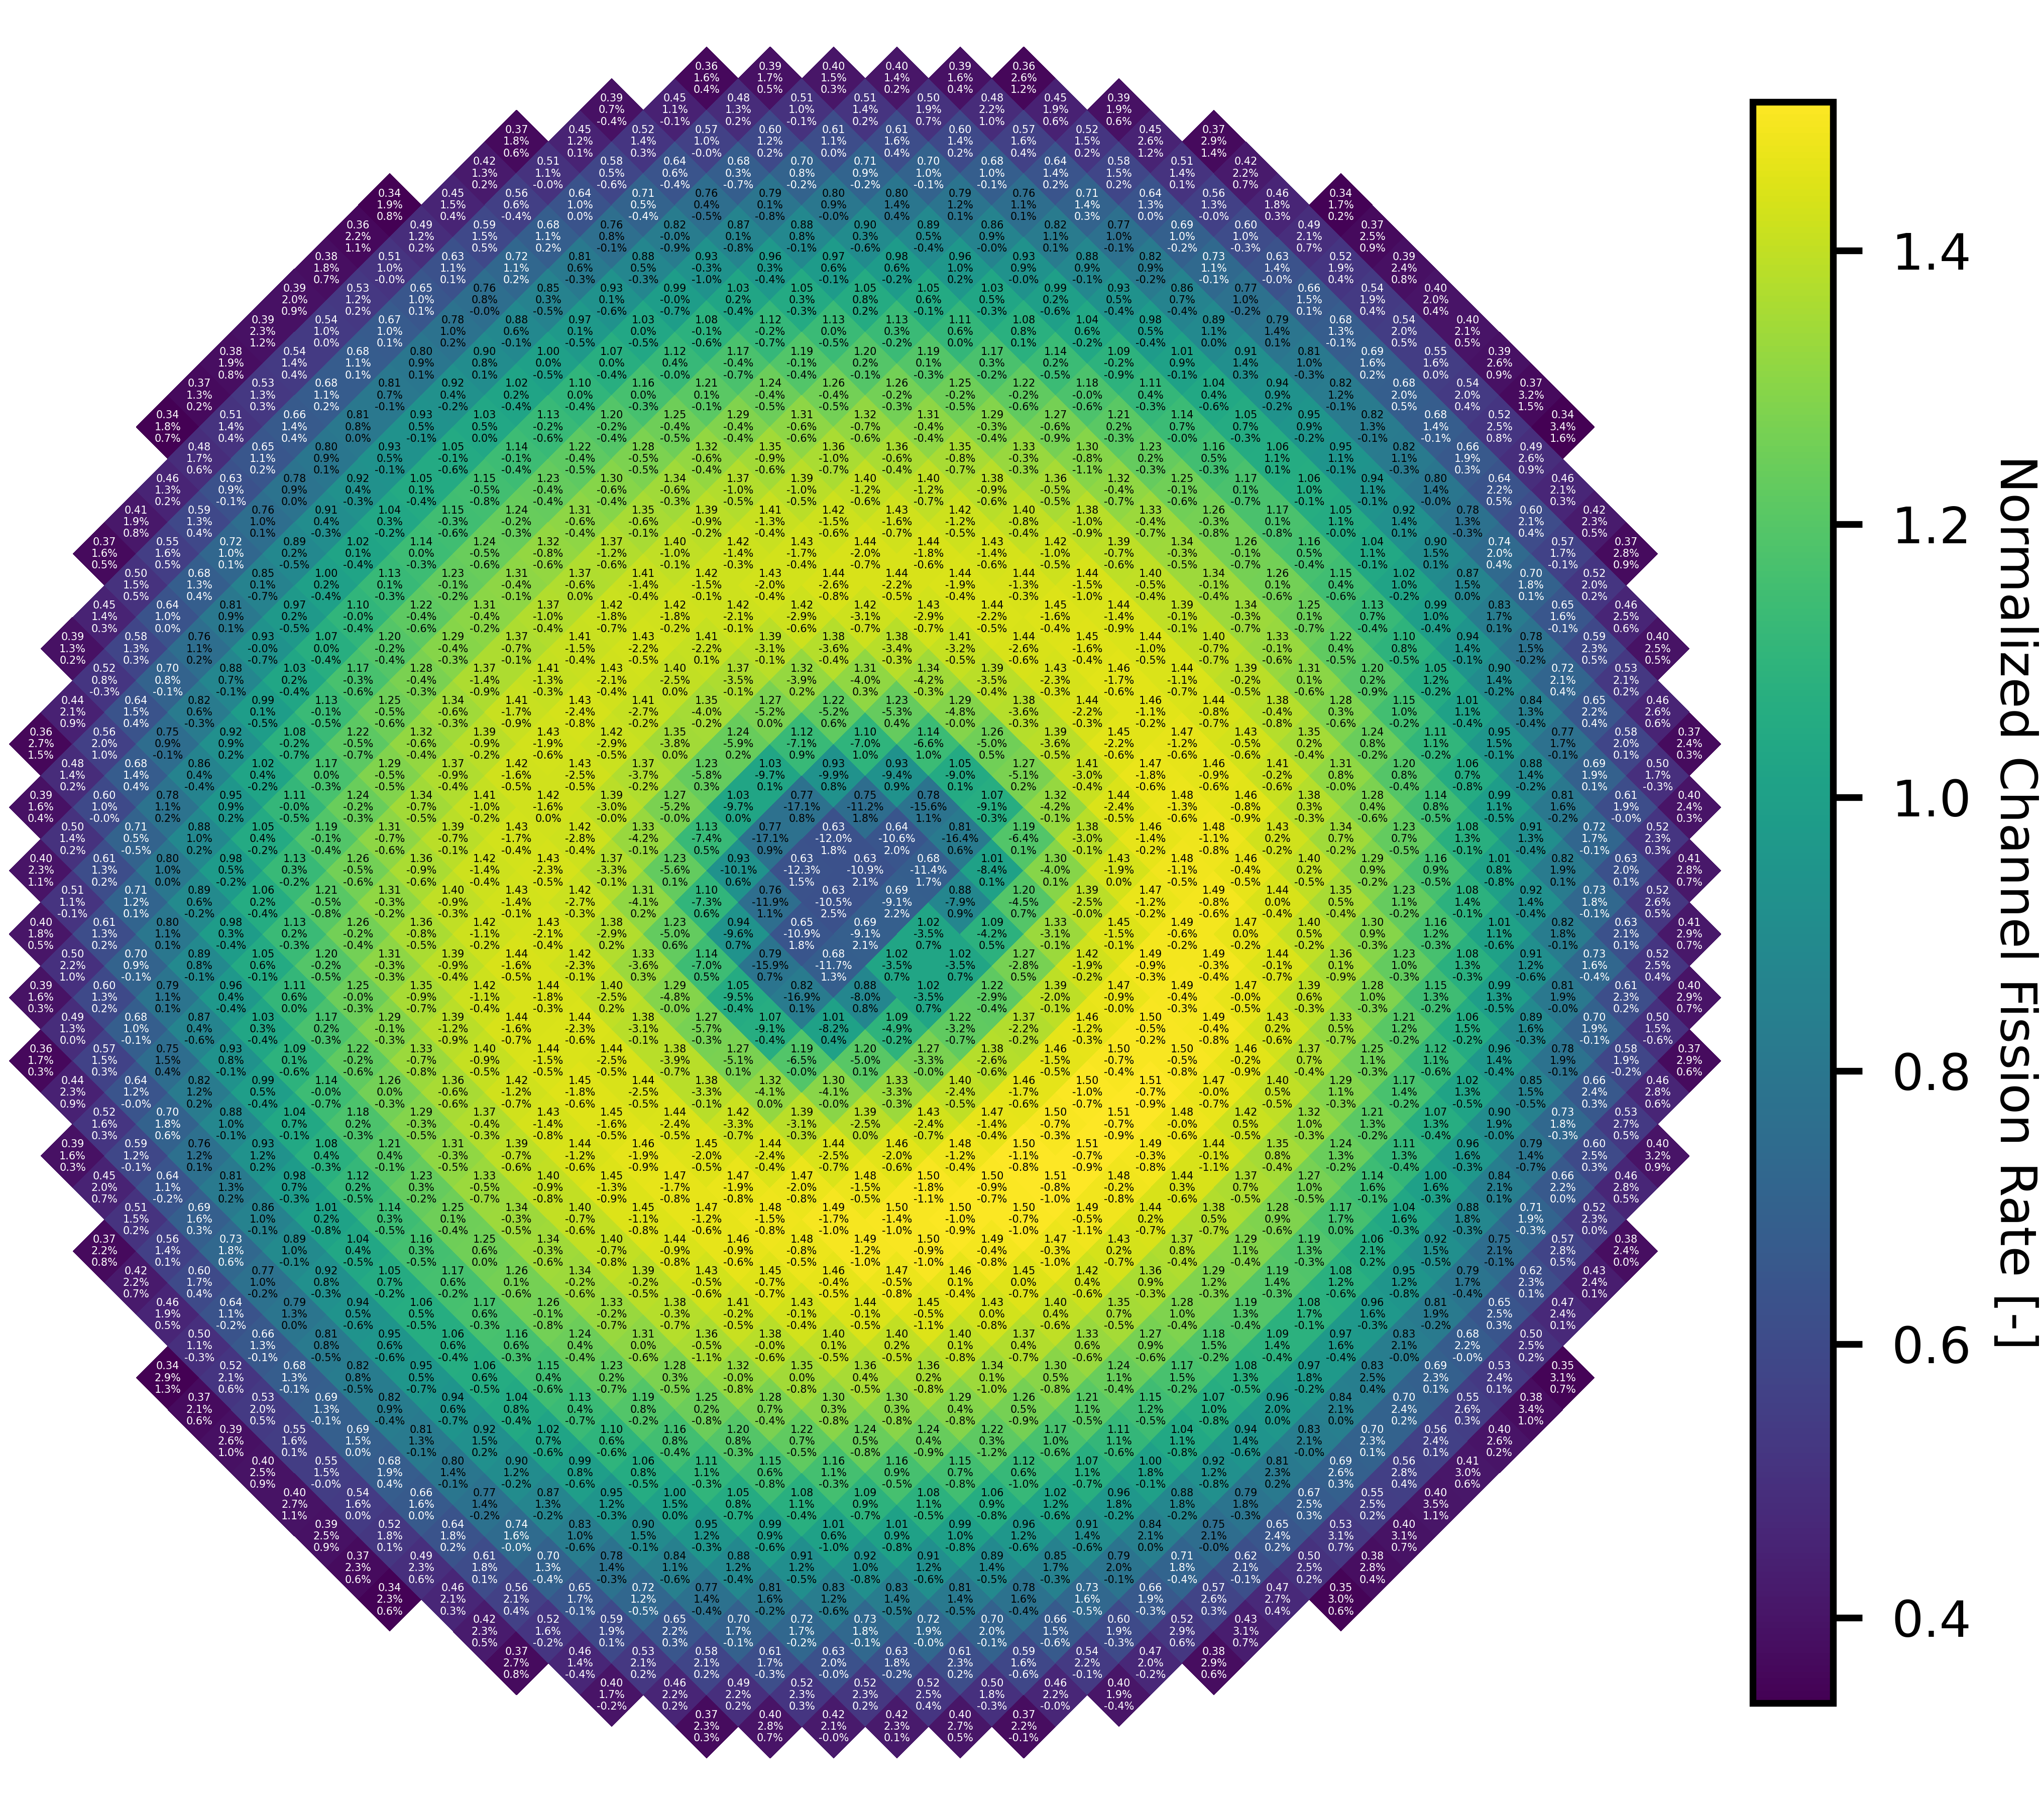
\includegraphics[width = .4\textwidth]{img/msre-full-123-power.png}
            
            \figcaption{
                    MSRE full core scalar flux error as calculated with pure diffusion, $S_N-D$,
                    and OpenMC for all control rods removed (left) and all control rods inserted (right)
            }
        }
    \end{tcolorbox}

    %%%%%%%%%%%%%%%%%%%%%%%%%%%%%%%%
    %%%%%%%%% OpenMCyclus %%%%%%%%%%
    %%%%%%%%%%%%%%%%%%%%%%%%%%%%%%%%
    \begin{tcolorbox}[colback=white, colframe=black, width=0.95\textwidth, arc=6pt, boxrule=1pt]
        \sectiontitle{OpenMCyclus}
        \sectioncontent{
            Reactor-physics informed fuel cycle analysis on the impacts of deploying HALEU-fueled reactors 
            using OpenMCyclus, a coupling of OpenMC with Cyclus \cite{bachmann}.

            \begin{minipage}{.45\textwidth}
                \vspace{1em}
                \includegraphics[width = \textwidth]{img/bachmann.jpg}
                \newline
                \figcaption{
                    Depletion methodology in OpenMCyclus. Blue comes from Cyclus and Red is 
                    provided through user-inputs.
                }
            \end{minipage}
            \hspace{1cm}
            \begin{minipage}{.45\textwidth}
                \vspace{1em}
                \includegraphics[width = \textwidth]{img/comparison_pu_cumulative.pdf}
                \newline
                \figcaption{
                    Comparison of the cumulative mass of separated plutonium traded after 
                    using the OpenMCyclus and Cycamore reactor.
                }
            \end{minipage}
        }
    \end{tcolorbox}

    %%%%%%%%%%%%%%%%%%%%%%%%%%%%%%%%%
    %%%%%%%%%%%%% ROLLO %%%%%%%%%%%%%
    %%%%%%%%%%%%%%%%%%%%%%%%%%%%%%%%%
    \begin{tcolorbox}[colback=white, colframe=black, width=0.95\textwidth, arc=6pt, boxrule=1pt]
        \sectiontitle{ROLLO}
        \sectioncontent{
            Evolutionary algorithm techniques applied to optimize nuclear reactor design by coupling 
            nuclear software to the DEAP evolutionary algorithm driver \cite{chee}.

            \includegraphics[width = .7\textwidth]{img/assem-obj-3-2d.png}
            \newline
            \figcaption{
                Triple-objective optimization to minimize total fuel packing fraction, max temp, and 
                fuel-normalized power peaking factor in the one-third assembly.
            }
        }
    \end{tcolorbox}

    %%%%%%%%%%%%%%%%%%%%%%%%%%%%%%%%%
    %%%%%% Logos (UIUC, ARFC) %%%%%%%
    %%%%%%%%%%%%%%%%%%%%%%%%%%%%%%%%%
    \includegraphics[height=0.28\textwidth]{img/UIUC_Logo.png}\hspace{5cm}
    \includegraphics[height=0.28\textwidth, trim={0 .5cm 0 .5cm}]{img/arfc_atom.png}

\end{center}